
% Бүлэг 2
\chapter{Системийн шинжилгээ ба зохиомж} % Бүлгийн нэр
\label{Chapter2} % Энэ бүлэг рүү ишлэл хийх бол \ref{Chapter2} командыг ашигла 

\section{Системийн үйл ажиллагааны тухай дэлгэрэнгүй}

\qquad
Энэхүү систем нь хэрэглэгчийн пиццаны захиалгыг утсаар хүлээн авахаас эхлээд захиалга бүртгэх, үнийн дүн болон хөнгөлөлт тооцох, хүргэгчид хуваарилах, төлбөр хүлээн авах, баримтыг баталгаажуулах, захиалгыг хаах хүртэлх бүх үйл ажиллагааг удирдана.

Үндсэн захиалгыг утсаар авч, захиалга хүлээн авагч системд бүртгэнэ. Цаашид вэбсайт эсвэл гар утасны апп нэмбэл хэрэглэгчийн оруулсан захиалга мөн адил энэхүү үндсэн процесс руу автоматаар орж болно.

\begin{figure}
    \centering
    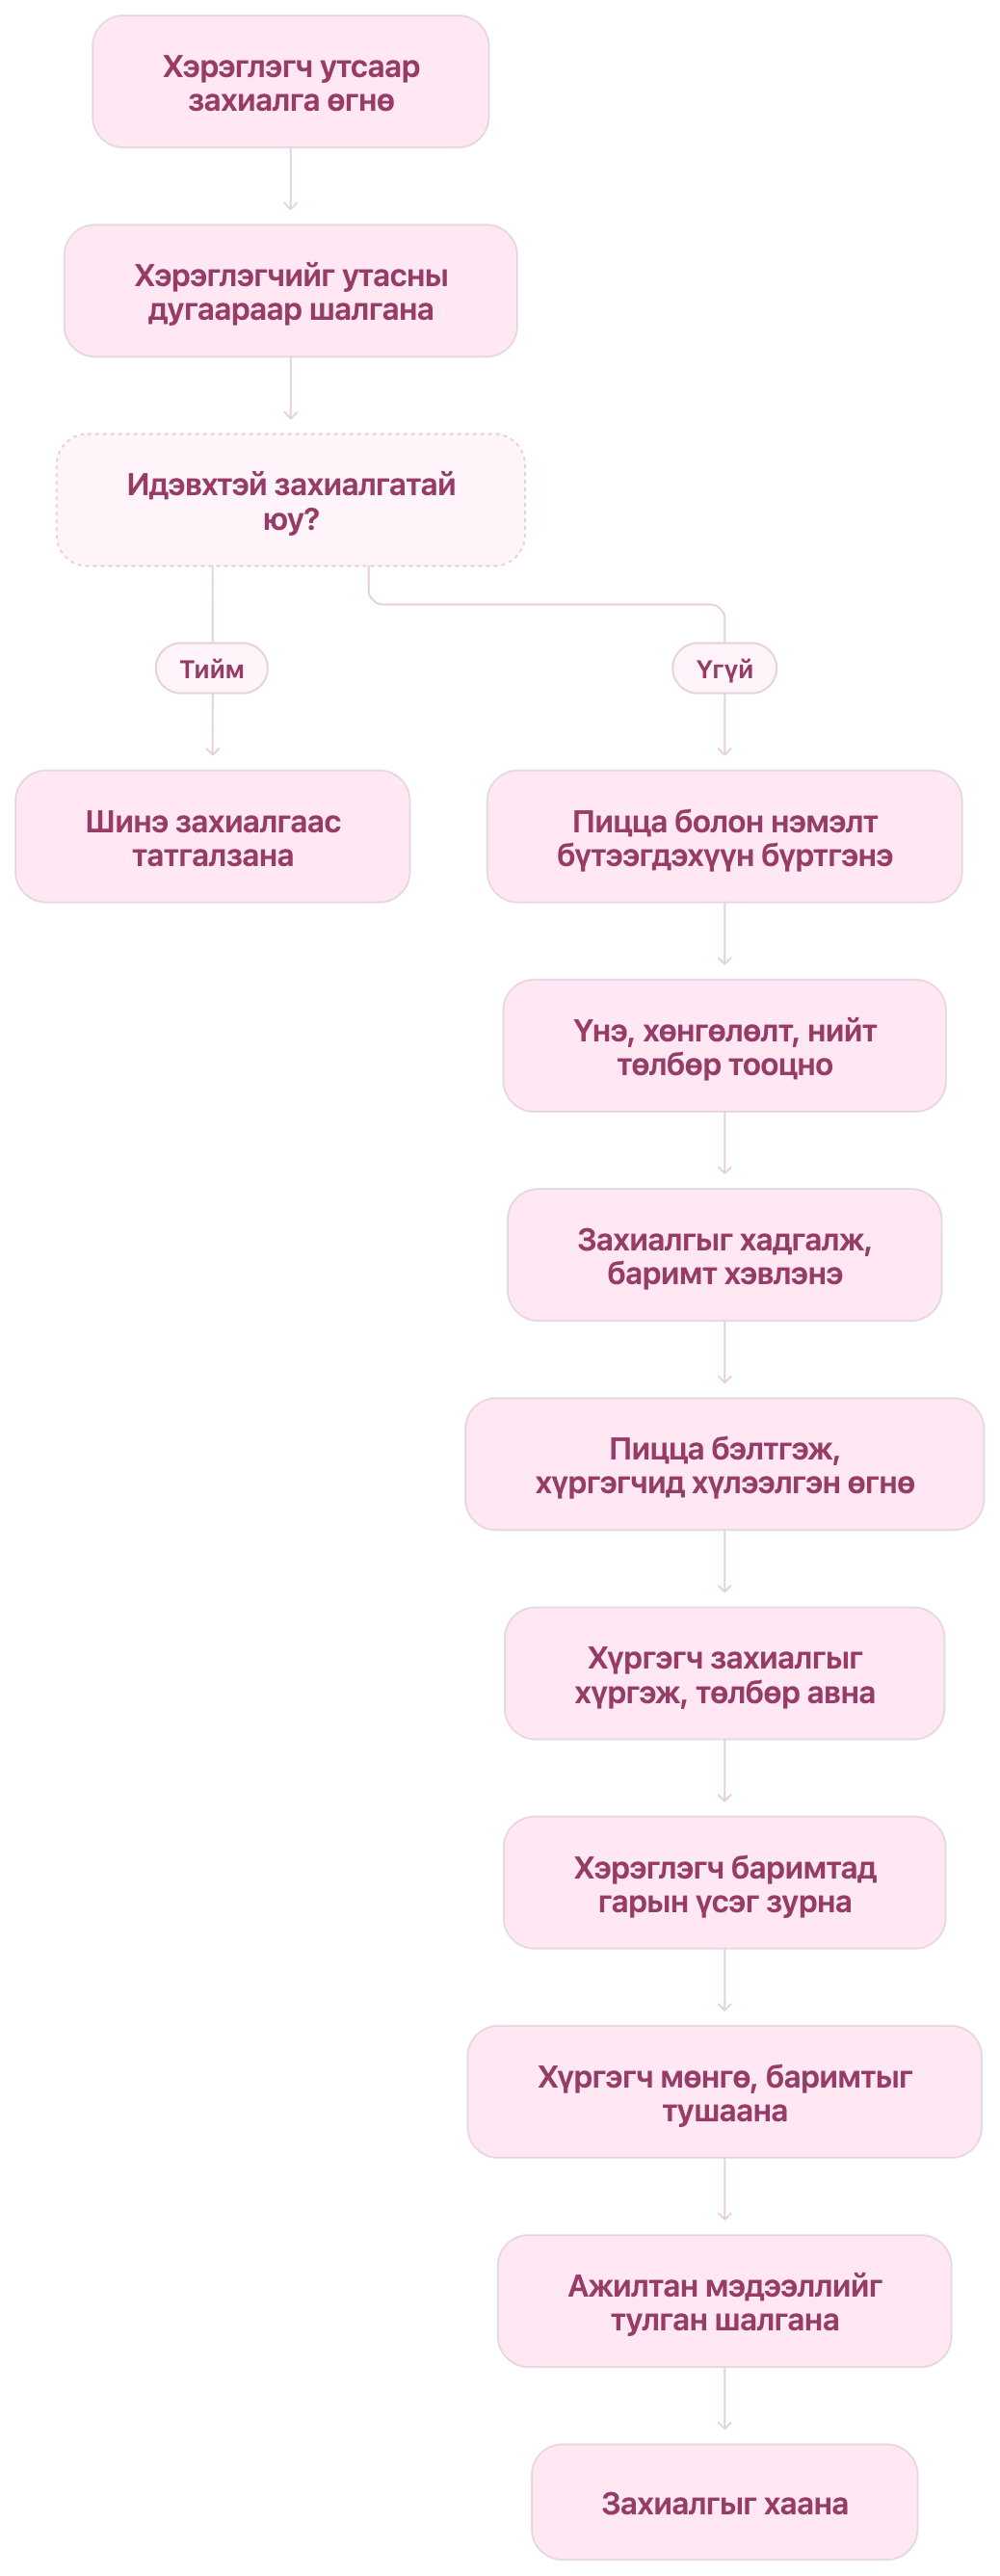
\includegraphics[width=0.65\linewidth]{mermaid-diagram.png}
    \caption{Үндсэн үйл ажиллагааны дараалал}
    \label{fig:placeholder}
\end{figure}


\section{Системийн хамрах хүрээ}
Системийн үндсэн хэрэглэгчид дараах байдлаар байх бөгөөд тэдгээрийн үүргүүдийг дурьдвал

\begin{enumerate}
    \item \textbf{Захиалга хүлээн авагч / бүртгэгч:} 
    Утасны захиалга авах, захиалагчийг шалгах, захиалга бүртгэх, баримт хэвлэх, хүргэгчид захиалга хуваарилах, мөнгө болон гарын үсэгтэй баримтыг хүлээн авч захиалгыг хаах

    \item \textbf{Хүргэгч:} 
    Хүргэлтийн мэдээлэл харах, пицца ба баримт хүлээн авах, захиалгыг хүргэх, төлбөр хураах, хүргэлтийн үр дүнг бүртгэх, мөнгө ба баримтыг тушаах

    \item \textbf{Системийн администратор:} 
    Хэрэглэгчийн бүртгэл болон эрх удирдах, бүтээгдэхүүн, үнэ, хөнгөлөлтийн нөхцөл тохируулах, системийн ажиллагааг хянах

    \item \textbf{Менежер / удирдлага:} 
    Захиалга, борлуулалт, хөнгөлөлт, хүргэлт, төлбөрийн тайлан харах, үйл ажиллагаанд хяналт тавих

\end{enumerate}
Гадаад оролцогчоор Захиалагч байх бөгөөд утсаар захиалга өгч, пицца хүлээн авч, төлбөр төлөн, баримтад гарын үсэг зурна. Гэхдээ системд шууд нэвтрэхгүй тул системийн шууд хэрэглэгч биш, харин бизнес процессын оролцогч юм.

\section{Хэрэглэгчийн шаардлага}

\textbf{1. Захиалга хүлээн авах буюу захиалга бүртгэх функц}
Хэрэглэгч байгууллагын утасны дугаар руу залгаж захиалга өгнө. Захиалга хүлээн авагч системд өөрийн хэрэглэгчийн нэр, нууц үгээр нэвтэрсэн байна.

Захиалга хүлээн авагч хэрэглэгчээс дараах мэдээллийг авна:
\begin{itemize}
    \item нэр;
    \item утасны дугаар;
    \item хүргэлтийн хаяг;
    \item орц, байр, давхар, тоот;
    \item нэмэлт тайлбар;
    \item захиалах бүтээгдэхүүн;
    \item пиццаны төрөл;
    \item пиццаны хэмжээ;
    \item гурилын төрөл;
    \item тоо ширхэг;
    \item нэмэлт орц;
    \item ундаа болон бусад бүтээгдэхүүн;
    \item төлбөрийн хэлбэр.
\end{itemize}

Утасны дугаар нь захиалагчийг таних үндсэн мэдээлэл байна. Системд өмнө нь бүртгэгдсэн хэрэглэгч бол нэр, утас, хүргэлтийн хаягийг автоматаар харуулна. Захиалга хүлээн авагч мэдээллийг шалгаж, шаардлагатай бол шинэчилнэ.

Шинэ хэрэглэгч бол системд хэрэглэгчийн шинэ бүртгэл үүсгэнэ.

\textbf{2. Идэвхтэй захиалгыг шалгах}

Шинэ захиалга үүсгэхээс өмнө систем тухайн утасны дугаартай хэрэглэгчид идэвхтэй захиалга байгаа эсэхийг автоматаар шалгана.

Дараах төлөвтэй захиалгыг идэвхтэйд тооцно:

\begin{itemize}
    \item шинээр бүртгэгдсэн;
    \item баталгаажсан;
    \item бэлтгэгдэж байгаа;
    \item хүргэгчид хуваарилсан;
    \item хүргэлтэд гарсан;
    \item хүргэгдсэн боловч төлбөр тооцоо дуусаагүй;
    \item мөнгө, баримт хүлээгдэж байгаа.
\end{itemize}

Хэрэв хэрэглэгч идэвхтэй захиалгатай бол систем шинэ захиалга хадгалахыг хориглож: \\
“Энэ хэрэглэгчид хаагдаагүй захиалга байна. Өмнөх захиалгыг хаасны дараа шинэ захиалга бүртгэнэ үү.” гэсэн мэдээлэл харуулна.

Хаагдсан болон цуцлагдсан захиалгыг идэвхтэйд тооцохгүй. Ийм хэрэглэгч дахин захиалга өгөх боломжтой.

\textbf{3. Бүтээгдэхүүн сагслах буюу бүтээгдэхүүн сонгох}

Захиалга хүлээн авагч системийн бүтээгдэхүүний жагсаалтаас хэрэглэгчийн сонгосон бүтээгдэхүүнийг сонгоно.

Бүтээгдэхүүн бүр дараах мэдээлэлтэй байна:

\begin{itemize}
    \item бүтээгдэхүүний код;
    \item бүтээгдэхүүний нэр;
    \item ангилал;
    \item хэмжээ;
    \item үндсэн үнэ;
    \item нэмэлт орцын үнэ;
    \item худалдаанд байгаа эсэх;
    \item бэлтгэх боломжтой салбар;
    \item орц, найрлага;
    \item харшил үүсгэж болзошгүй орц.
\end{itemize}

Нэг захиалгад хэд хэдэн төрлийн пицца, ундаа болон нэмэлт бүтээгдэхүүн оруулж болно. Систем бүтээгдэхүүн бүрийн тоо ширхэг болон үнийг үржүүлж мөрийн дүнг автоматаар тооцно.

$$ \text{Мөрийн дүн}=\text{Нэгж үнэ}\times\text{Тоо ширхэг} $$

Бүх бүтээгдэхүүний мөрийн дүнгийн нийлбэрээр захиалгын анхны нийт үнийг олно.

$$ \text{Анхны нийт үнэ}=\sum \text{Бүтээгдэхүүний мөрийн дүн} $$

\textbf{4. Хөнгөлөлт тооцох}

Систем захиалгын анхны нийт үнийг тооцсоны дараа хөнгөлөлтийн нөхцөлийг шалгана.

Бизнесийн үндсэн дүрэм:

\begin{enumerate}
    \item анхны нийт үнэ 40,000 төгрөгөөс дээш бол 20 хувийн хөнгөлөлт олгоно;
    \item анхны нийт үнэ 40,000 төгрөгтэй тэнцүү бол хөнгөлөлт олгохгүй;
    \item анхны нийт үнэ 40,000 төгрөгөөс бага бол хөнгөлөлт олгохгүй.
\end{enumerate}


$$ \text{Хөнгөлөлт}= \begin{cases} \text{Анхны нийт үнэ}\times 0.20, & \text{нийт үнэ}>40,000\\ 0, & \text{нийт үнэ}\leq40,000 \end{cases} $$ $$ \text{Төлөх дүн}=\text{Анхны нийт үнэ}-\text{Хөнгөлөлт} $$

Жишээлбэл, захиалгын анхны нийт үнэ 50,000 төгрөг бол:

$$ 50,000\times20\%=10,000 $$ $$ 50,000-10,000=40,000 $$

Иймд хэрэглэгч 40,000 төгрөг төлнө.

Систем дараах дүнг тусад нь харуулна:

\begin{itemize}
    \item барааны нийт үнэ;
    \item хөнгөлөлтийн хувь;
    \item хөнгөлөлтийн дүн;
    \item хүргэлтийн төлбөр;
    \item төлөх эцсийн дүн.
\end{itemize}

Хүргэлтийн төлбөрийг хөнгөлөлт тооцох анхны үнэд оруулах эсэхийг байгууллагын бизнесийн дүрмээр тусад нь тодорхойлох шаардлагатай.

\textbf{5. Захиалгыг баталгаажуулах}

Мэдээллийг бүрэн оруулсны дараа захиалга хүлээн авагч хэрэглэгчид дараах мэдээллийг дахин уншиж баталгаажуулна:

\begin{itemize}
    \item сонгосон бүтээгдэхүүн;
    \item тоо ширхэг;
    \item нэмэлт орц;
    \item хүргэлтийн хаяг;
    \item анхны үнэ;
    \item хөнгөлөлт;
    \item хүргэлтийн төлбөр;
    \item төлөх эцсийн дүн;
    \item хүргэлтийн ойролцоо хугацаа.
\end{itemize}

Хэрэглэгч зөвшөөрсний дараа ажилтан “Захиалга баталгаажуулах” үйлдлийг сонгоно.

Систем захиалгад давтагдашгүй дугаар үүсгэнэ. Жишээлбэл:

ORD-20260922-00125

Захиалгын анхны төлөв “Бүртгэгдсэн” болно. Систем захиалгыг бүртгэсэн ажилтан, огноо, цагийг автоматаар хадгална.

\textbf{6. Гал тогоонд шилжүүлэх}

Баталгаажсан захиалгыг гал тогоо эсвэл пицца бэлтгэх хэсэгт шилжүүлнэ. Гал тогооны ажилтан дэлгэц эсвэл хэвлэсэн хуудсаас дараах мэдээллийг харна:

\begin{itemize}
    \item захиалгын дугаар;
    \item бүтээгдэхүүний нэр;
    \item хэмжээ;
    \item тоо ширхэг;
    \item нэмэлт болон хасах орц;
    \item хэрэглэгчийн тусгай хүсэлт;
    \item захиалга бүртгэсэн цаг;
    \item бэлэн болгох зорилтот хугацаа.
\end{itemize}

Гал тогоо захиалгыг хүлээн авсны дараа төлөвийг “Бэлтгэгдэж байгаа” болгон өөрчилнө. Пицца бэлэн болсон үед “Бэлэн болсон” төлөвт оруулна.

Бэлтгэх боломжгүй бүтээгдэхүүн илэрвэл захиалга хүлээн авагч хэрэглэгчтэй холбогдож:

\begin{enumerate}
    \item бүтээгдэхүүнийг өөр бүтээгдэхүүнээр солих;
    \item тоо ширхэгийг өөрчлөх;
    \item захиалгын тухайн мөрийг хасах;
    \item захиалгыг бүхэлд нь цуцлах
\end{enumerate}

шийдвэрийн аль нэгийг бүртгэнэ.

\textbf{7. Хүргэгчид захиалга хуваарилах}

Пицца бэлэн болсны дараа захиалга хүлээн авагч эсвэл хүргэлтийн зохицуулагч боломжтой хүргэгчээс сонгоно.

Систем хүргэгч бүрийн дараах мэдээллийг харуулж болно:

\begin{itemize}
    \item хүргэгчийн нэр;
    \item утасны дугаар;
    \item ажиллаж байгаа эсэх;
    \item одоогийн захиалгын тоо;
    \item хүргэлтэд гарсан цаг;
    \item хүргэлтийн бүс;
    \item төлөв.
\end{itemize}

Захиалгыг хүргэгчид хуваарилсны дараа хүргэлтийн баримт хэвлэнэ. Баримтад дараах мэдээлэл байна:

\begin{itemize}
    \item байгууллагын нэр;
    \item захиалгын дугаар;
    \item захиалгын огноо, цаг;
    \item захиалагчийн нэр;
    \item утасны дугаар;
    \item хүргэлтийн хаяг;
    \item бүтээгдэхүүний жагсаалт;
    \item бүтээгдэхүүн бүрийн үнэ;
    \item анхны нийт үнэ;
    \item хөнгөлөлтийн дүн;
    \item хүргэлтийн төлбөр;
    \item төлөх эцсийн дүн;
    \item хүргэгчийн нэр;
    \item хэрэглэгчийн гарын үсэг зурах хэсэг;
    \item хүргэгчийн гарын үсгийн хэсэг;
    \item тусгай тайлбар.
\end{itemize}

Захиалга, пицца болон баримтыг хүргэгч хүлээн авсны дараа системийн төлөвийг “Хүргэлтэд гарсан” болгон өөрчилнө. Хүргэлтэд гарсан огноо, цагийг автоматаар бүртгэнэ.

\textbf{8. Захиалгыг хүргэх}

Хүргэгч баримт болон пиццаг захиалагчийн хаягт хүргэнэ. Хэрэглэгч захиалгаа шалгасны дараа төлбөрийг хүргэгчид өгнө.

Хүргэгч дараах үйлдлийг гүйцэтгэнэ:

\begin{enumerate}
    \item Захиалагчийн нэр, утас, хаягийг тулган шалгах.
    \item Бүтээгдэхүүнийг хэрэглэгчид хүлээлгэн өгөх.
    \item Төлөх эцсийн дүнг баримттай тулгах.
    \item Төлбөрийг бэлэн мөнгөөр хүлээн авах.
    \item Шаардлагатай бол хариулт мөнгө өгөх.
    \item Хэрэглэгчээр хүргэлтийн баримтад гарын үсэг зуруулах.
    \item Хүргэлтийн үр дүнг системд бүртгэх.
\end{enumerate}

Амжилттай хүргэсэн бол захиалгын төлөв “Хүргэгдсэн” болно.

Системд дараах мэдээллийг хадгална:

\begin{itemize}
    \item бодитоор хүлээн авсан мөнгө;
    \item хариулт мөнгө;
    \item хүргэж дууссан цаг;
    \item гарын үсэг авсан эсэх;
    \item хүргэлтийн тайлбар;
    \item хүргэлтийн үр дүн.
    \item 10. Хүргэлт амжилтгүй болох
\end{itemize}

Дараах тохиолдолд хүргэлт амжилтгүй болж болно:

\begin{itemize}
    \item захиалагч утсаа авахгүй байх;
    \item хаяг буруу эсвэл тодорхойгүй байх;
    \item захиалагч заасан хаягт байхгүй байх;
    \item захиалагч захиалга өгөөгүй гэж мэдэгдэх;
    \item захиалагч бүтээгдэхүүнээс татгалзах;
    \item төлбөр хүрэлцэхгүй байх;
    \item хүргэлтийн явцад бүтээгдэхүүн гэмтэх;
    \item цаг агаар, замын нөхцөлөөс шалтгаалан хүргэх боломжгүй болох.
\end{itemize}

Энэ үед хүргэгч “Хүргэлт амжилтгүй” төлөв сонгож, шалтгааныг заавал бүртгэнэ. Захиалга хүлээн авагч хэрэглэгчтэй холбогдон:

\begin{itemize}
    \item дахин хүргэх;
    \item хаягийг засах;
    \item бүтээгдэхүүнийг дахин бэлтгэх;
    \item захиалгыг цуцлах
\end{itemize}

шийдвэр гаргана.

Цуцлагдсан захиалгад цуцалсан ажилтан, шалтгаан, огноо, цагийг хадгална.

\textbf{10. Мөнгө болон баримт тушаах}

Хүргэлт дууссаны дараа хүргэгч байгууллагад буцаж ирэн дараах зүйлсийг захиалга хүлээн авагчид тушаана:

\begin{itemize}
    \item хэрэглэгчээс хүлээн авсан мөнгө;
    \item хэрэглэгчийн гарын үсэгтэй баримт;
    \item амжилтгүй хүргэлтийн бүтээгдэхүүн, хэрэв байгаа бол;
    \item хүргэлтийн нэмэлт тайлбар.
\end{itemize}

Захиалга хүлээн авагч систем дэх төлөх дүнг хүргэгчийн тушаасан мөнгөтэй тулгана.

$$ \text{Зөрүү}=\text{Тушаасан мөнгө}-\text{Системийн төлөх дүн} $$

Зөрүү тэгтэй тэнцүү бол төлбөрийг зөв гэж үзнэ. Зөрүү гарвал систем захиалгыг шууд хаахгүй бөгөөд:

\begin{itemize}
    \item илүү мөнгө;
    \item дутуу мөнгө;
    \item баримт ирээгүй;
    \item гарын үсэг байхгүй;
    \item баримт гэмтсэн
\end{itemize}
гэсэн шалтгааны аль нэгийг бүртгэнэ.

Мөнгө болон баримтыг хүлээн авсны дараа захиалгын төлөвийг “Тооцоо шалгагдаж байгаа” болгоно.

\textbf{11. Захиалгыг хаах}

Захиалгыг хаахаас өмнө систем дараах нөхцөлийг шалгана:

\begin{itemize}
    \item захиалга хүргэгдсэн байх;
    \item төлбөр бүрэн хүлээн авсан байх;
    \item тушаасан мөнгө төлөх дүнтэй тохирсон байх;
    \item гарын үсэгтэй баримт буцаан ирсэн байх;
    \item хүргэгч мөнгө, баримтаа тушаасан байх;
    \item шаардлагатай төлбөрийн баримт үүссэн байх.
\end{itemize}

Бүх нөхцөл хангагдсан бол захиалга хүлээн авагч “Захиалга хаах” үйлдлийг сонгоно. Систем захиалгын төлөвийг “Хаагдсан” болгон өөрчилж, хаасан ажилтан, огноо, цагийг хадгална.

Хаагдсан захиалгыг энгийн хэрэглэгч өөрчлөх боломжгүй. Зөвхөн эрх бүхий администратор үндэслэл бүхий засвар хийж болох бөгөөд бүх өөрчлөлтийг аудитын бүртгэлд хадгална.

Захиалга хаагдсаны дараа тухайн хэрэглэгч шинэ захиалга өгөх боломжтой болно.

\section{Функциональ шаардлага}

\textbf{Захиалга хүлээн авагчийн функциональ шаардлага}
\begin{enumerate}
    \item захиалагчийг хайх, бүртгэх;
    \item идэвхтэй захиалга шалгах;
    \item захиалга үүсгэх, засах;
    \item бүтээгдэхүүн сонгох;
    \item хөнгөлөлт шалгах;
    \item хүргэгч хуваарилах;
    \item баримт хэвлэх;
    \item мөнгө, баримт хүлээн авах;
    \item захиалга хаах.
\end{enumerate}

\textbf{Хүргэгчийн функциональ шаардлага}
\begin{itemize}
    \item өөрт хуваарилсан захиалгыг харах;
    \item пицца болон баримт хүлээн авах;
    \item хүргэлтэд гарсныг бүртгэх;
    \item хүргэлтийн үр дүн оруулах;
    \item төлбөрийн дүн бүртгэх;
    \item мөнгө, баримт тушаах.
\end{itemize}

\textbf{Менежерийн функциональ шаардлага}
\begin{itemize}
    \item бүх захиалга харах;
    \item хөнгөлөлтийн дүрэм тохируулах;
    \item хүргэлтийн ажиллагааг хянах;
    \item мөнгөний зөрүү шалгах;
    \item борлуулалтын тайлан харах;
    \item цуцлалт болон буцаалтыг батлах.
\end{itemize}
    
\textbf{Системийн администраторын функциональ шаардлага}
\begin{itemize}
    \item хэрэглэгчийн бүртгэл үүсгэх;
    \item хэрэглэгчийн эрх тохируулах;
    \item бүтээгдэхүүн, үнэ удирдах;
    \item системийн тохиргоо хийх;
    \item аудитын бүртгэл харах;
    \item мэдээллийн нөөцлөлт, хамгаалалтыг удирдах.
\end{itemize}

\textbf{Тайлангийн үйл ажиллагаа}

Систем дараах тайланг гаргах боломжтой байна:
\begin{itemize}
    \item өдөр, долоо хоног, сарын борлуулалт;
    \item нийт захиалгын тоо;
    \item хаагдсан болон цуцлагдсан захиалга;
    \item хөнгөлөлттэй захиалгын тоо, дүн;
    \item хамгийн их борлуулалттай бүтээгдэхүүн;
    \item хүргэгч бүрийн хүргэлтийн тоо;
    \item хүргэлтийн дундаж хугацаа;
    \item амжилтгүй хүргэлтийн шалтгаан;
    \item бэлэн мөнгөний орлого;
    \item мөнгөний илүү, дутуу зөрүү;
    \item хэрэглэгчийн гомдол;
    \item давтан захиалгын мэдээлэл.
\end{itemize}

\subsection{Системийн үндсэн бизнес дүрэм}
\begin{itemize}
    \item Нэг хэрэглэгч нэгэн зэрэг нэг л идэвхтэй захиалгатай байна.
    \item 40,000 төгрөгөөс дээш захиалгад 20 хувийн хөнгөлөлт олгоно.
    \item Хөнгөлөлтийг систем автоматаар тооцно.
    \item Хөнгөлөлтийг энгийн ажилтан гараар өөрчлөх боломжгүй байна.
    \item Захиалга бүр давтагдашгүй дугаартай байна.
    \item Хүргэгч зөвхөн өөрт хуваарилсан захиалгыг харна.
    \item Хүргэлтэд гарсан захиалгын бүтээгдэхүүн, үнийг зөвшөөрөлгүй өөрчлөхгүй.
    \item Мөнгө болон гарын үсэгтэй баримт ирээгүй бол захиалгыг хаахгүй.
    \item Төлбөрийн дүн зөрүүтэй бол захиалгыг хаахгүй.
    \item Зөвхөн эрх бүхий ажилтан захиалгыг цуцлах болон хаах боломжтой.
    \item Захиалгын төлөвийн өөрчлөлт бүрийг аудитын бүртгэлд хадгална.
    \item Хаагдсан захиалгыг зассан бүх тохиолдолд шалтгаан заавал бичнэ.
\end{itemize}

Ингэснээр систем нь захиалга бүртгэх энгийн программаас илүүтэйгээр захиалагч, захиалга хүлээн авагч, гал тогоо, хүргэгч, төлбөр тооцоо болон удирдлагыг нэг урсгалд холбосон нэгдсэн мэдээллийн систем болно

\section{Функционал бус шаардлага}

\subsection{Гүйцэтгэлийн шаардлага}
\begin{itemize}
    \item Хэрэглэгчдэд ойлгомжтой, энгийн интерфэйстэй байх.
    \item Дэлгэц шилжих хурд хамгийн ихдээ 10 секунд байх.
    \item Өвчтөний мэдээлэл болон эмийн мэдээлэл харах хурд 3-10 секунд байх.
    \item Өгөгдлийн сангийн ачаалал хурдан шуурхай байх.
\end{itemize}

\subsection{Аюулгүй байдлын шаардлага}
\begin{itemize}
    \item Сервер, өгөгдлийн сангийн аюулгүй байдлыг хангах.
    \item Өвчтөн, ажилтны мэдээлэл алдагдахгүй байх.
    \item Системийн нэвтрэлт зөвшөөрөгдсөн хэрэглэгчдэд зориулагдсан байх.
\end{itemize}

\subsection{Хамгаалалт, нууцлалын шаардлага}
\begin{itemize}
    \item Эмч, эмийн санч, хэрэглэгчийн мэдээллийг нууцлалтай хадгалах.
    \item Нууц үг дэлгэцэнд харуулахгүй байх.
    \item Сервер болон өгөгдлийн санг нууц хамгаалалттай байлгах.
\end{itemize}

\subsection{Программ хангамжийн чанарын шаардлага}
\begin{itemize}
    \item Ашиглахад хялбар, ойлгомжтой байх.
    \item Шинэчлэл хийх боломжтой байх.
    \item Монгол хэл дээр ажиллах.
    \item Систем нэгэн зэрэг олон хэрэглэгчийн хандалтыг дэмжих.
\end{itemize}

\section{Ашигласан технологи, техникийн шаардлага}

\subsection{Технологийн шаардлага}

\subsubsection{Программ ажиллах үйлдлийн системийн сонголт}
\qquad
Энэхүү эмийн систем нь мобайл болон вэб орчинд ажиллана. Мобайл үйл ажиллагааг дэмждэг бүх төхөөрөмж дээр веб браузерээр ажиллах боломжтой. Программ хангамжийн дэмжих үйлдлийн системүүд:

\begin{enumerate}
    \item Android үйлдлийн систем
    \item iOS үйлдлийн систем
    \item Windows үйлдлийн систем
    \item macOS үйлдлийн систем (заавал шаардлагатай бол)
\end{enumerate}

\subsubsection{Өгөгдлийн сангийн удирдах системийн сонголт}
\qquad
Энэхүү системийн өгөгдлийн сангийн баазыг MongoDB өгөгдлийн сан удирдах систем дээр хөгжүүлэхээр төлөвлөсөн. MongoDB нь NoSQL төрлийн өгөгдлийн сан бөгөөд дараах давуу талуудтай:

\begin{itemize}
    \item Их хэмжээний өгөгдлийг хурдан боловсруулж хадгалах
    \item Өвөрмөц бүтэцтэй өгөгдлийг хялбар удирдах
    \item Өндөр аюулгүй байдал, нөөцлөлт, сэргээх боломжтой
    \item Програмын хөгжүүлэлтэд уян хатан байдлыг хангах
\end{itemize}

\subsection{Техникийн шаардлага}
\subsubsection{Оролт гаралтын төхөөрөмжүүдийн шаардлага}

\begin{longtable}{| p{0.7cm} | p{4cm} | p{3.5cm} | p{3.3cm} |}
		\hline
		\textbf{№} & \textbf{Төхөөрөмж} & \textbf{Төрөл} & \textbf{Шаардлага}\\
		\hline
		1 & \begin{center}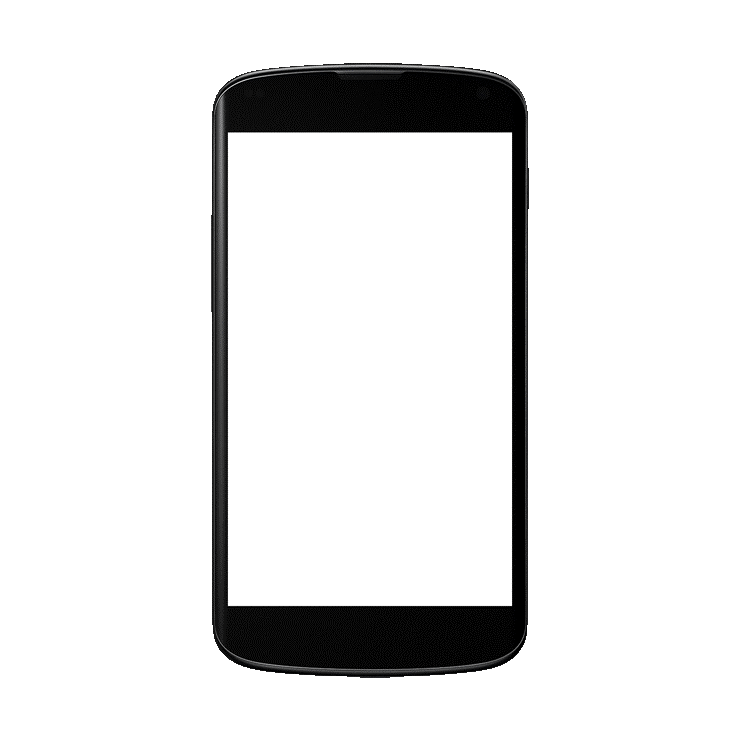
\includegraphics[width=2cm]{Figures/icon1} \end{center}& Мэдрэх & Энгийн  \\
		\hline
		2 & \begin{center}
\includegraphics[width=2cm]{Figures/icon2} \end{center} & Оролт & Энгийн \\
		\hline
		3 & \begin{center}
\includegraphics[width=2cm]{Figures/icon3} \end{center} & Гаралт & Дурын  \\
		\hline
		4 & \begin{center}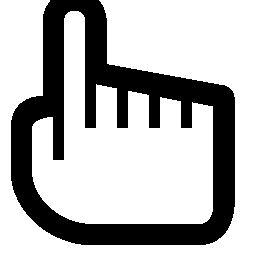
\includegraphics[width=2cm]{Figures/icon4} \end{center} & Заах & Дурын \\
		\hline
		\caption[Оролт гаралтын төхөөрөмжүүдийн шаардлага]{Оролт гаралтын төхөөрөмжүүдийн шаардлага}

	\end{longtable}


    

\section{Юзкейс диаграм}

....